\chapter{Activation Functions}\label{ch_act_functions}
\chapterauthor{Jeff Yoshimi, Scott Hotton}

% Consider formally setting off definitions

 As discussed in the introduction, artificial neural networks are comprised of nodes connected by weights. The nodes are usually pictured as circles and are associated with a number called an activation, while the weights are represented by lines connecting the nodes and are associated with a number called a strength. In Simbrain, node activations correspond to the colors of the nodes and to the number inside the nodes, and weight strengths correspond to the color and size of the filled disks at the end of the lines connecting nodes. In figure \ref{F:simplenet1} (Left), three nodes are connected to one node via three weights. 

When a neural network simulation is run, node activations and weight strengths change. Neural networks have \emph{dynamics}, which describe a changing pattern of activation across the nodes and (in some cases) a changing pattern of strengths of across the weights. To see these dynamics in Simbrain, look for the triangular ``play''  button 
\includegraphics[scale=.5]{./images/Play.png}. When you press it you usually see node activations change, and in some cases weight strengths. In this chapter we describe some of the rules that govern changing node activations.\footnote{When you open up a dialog to train a network, there is another play button that is used to modify the weights. When these buttons are pressed the dynamics of nodes and weights is simulated. In chapters \extref{ch_linear_algebra}, \extref{ch_unsupervised}, and \extref{ch_supervised}, we discuss the rules governing changes in weight strengths.} These are based loosely on the physiology of neurons and action potentials, which was discussed in chapter \extref{ch_neuro}. 

Rules for updating node activations make use of an \glossary{activation function}, which sets the activation of a node based on the values of incoming node activations and the weights connecting them together. These are classical rules that have been used in many kinds of simulations since the early days of neural networks. There are many other rules for updating neural networks--some geared more towards computational neuroscience, some towards engineering--but even today these classical rules are frequently used.\footnote{To get a sense of the diversity of functions available, try editing a few nodes in Simbrain and changing the 
``update rule" drop down box. As you change the selection, you will notice that 
the parameters available to you change. You can also wire together a small 
network and just see what happens when you use these rules. Several neurally realistic ``spiking'' activation rules are included in Simbrain, which are discussed further in chapter \extref{ch_spiking}.}

\begin{figure}[h]
\centering
\raisebox{-0.5\height}{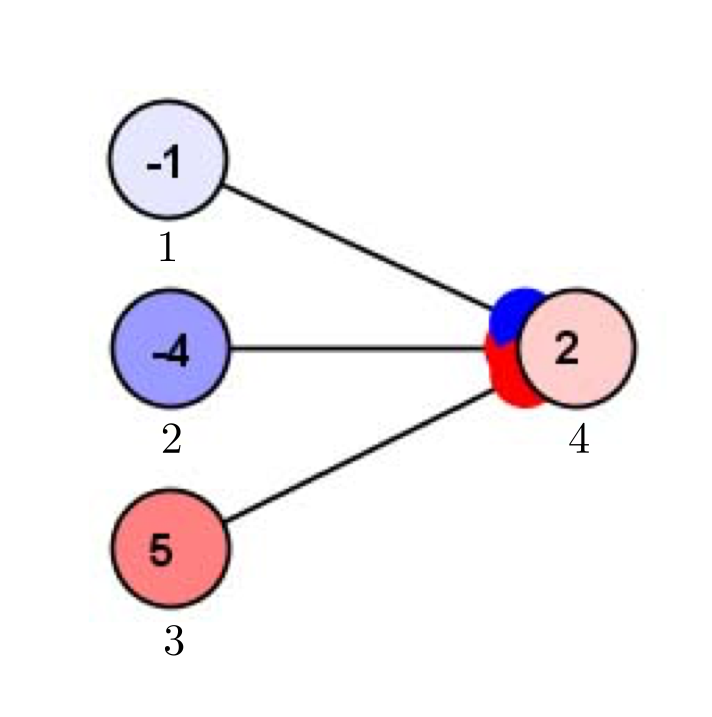
\includegraphics[scale=.7]{./images/Simple3Labelled.png}}
\hspace*{.4in}
\raisebox{-0.5\height}{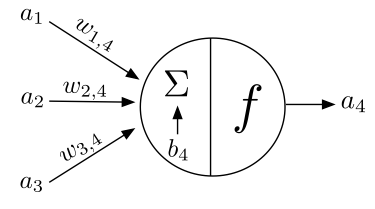
\includegraphics[scale=.7]{./images/activationFunction.png}}
\caption[Left: Simbrain screenshot; Right: Jeff Yoshimi.]{(Left) A simple neural network with three nodes attached to one node via three weights. (Right) Schematic of the same network to illustrate the notation being used here. Nodes $1,2, 3$ are connected to node $4$. In this example, $a_1 = -1$, $a_2 = -4$, $a_3=5$ and (though weight strengths are not visible) $w_{1,4} = -1$, $w_{2,4} = 1$, $w_{3,4} = 1$, $b_4 = 0$ and the activation function is linear with a slope of 1, so that $a_4 = 2$. $\Sigma$ represents the weighted inputs, and $f$ represents the activation function. A network like this is included with Simbrain as \emph{simpleNet.zip}}
\label{F:simplenet1}
\end{figure}
% Add x-y axis lines? 

\section{Weighted Inputs and Activation Functions}

 We will represent the activation of the $j^{\rm th}$ node of a network by $a_j$. The 
strength of the weight connecting the $j^{\rm th}$ node to the $k^{\rm th}$  node will be denoted by $w_{j,k}$. This notation is illustrated in figure \ref{F:simplenet1}. Activation $a_j$ of node $j$ is updated by first 
computing the \glossary{weighted input} to node $j$  (roughly: the weighted sum of activations from other incoming nodes) and then passing that value through an activation function denoted by $f$. The basic flow of operations is shown in figure \ref{F:simplenet1} (Right). In this section we discuss weighted inputs in more detail and then consider three of the most common forms for the activation function: threshold, 
linear, and sigmoid.
% The notation w_j,k is not always followed. Sometimes the opposite is used, where i is target and k is source. (ex. Matlab neural net docs). Faussett has a nice way of putting it.
% This is called a ``local field'' or ``activation potential'' by Haykin

\begin{figure}[h]
\centering
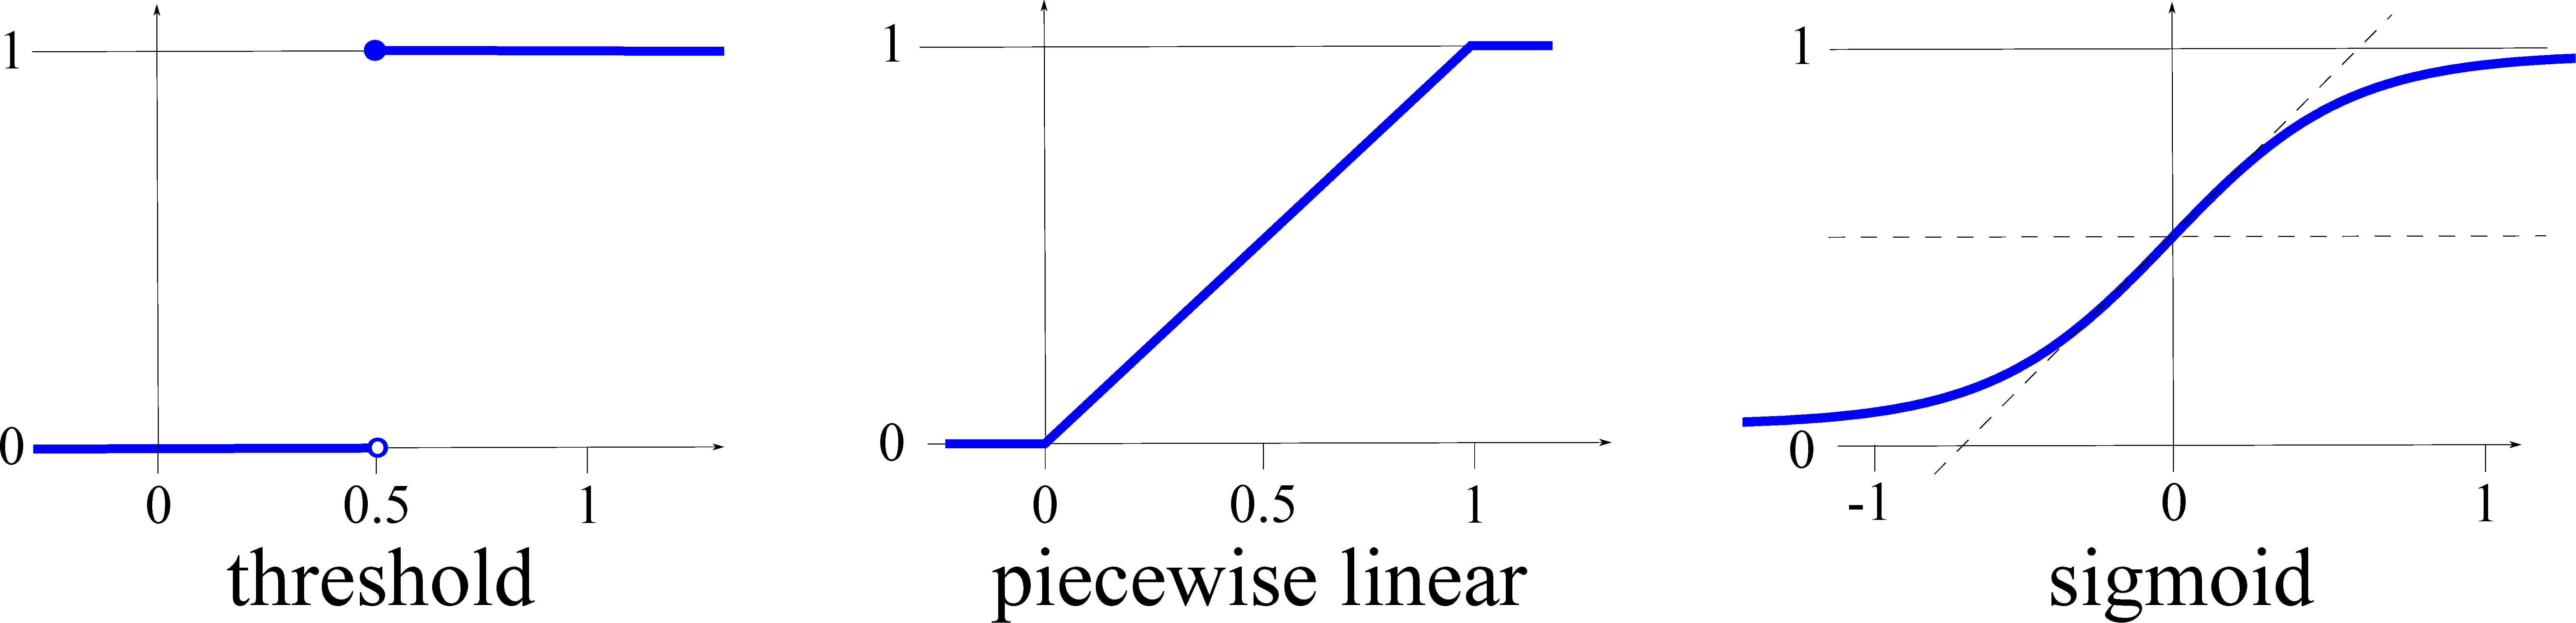
\includegraphics[scale=0.130]{./images/graph_binary.pdf}
\caption[Scott Hotton.]{The graphs for three activation functions. In each of the graphs, the 
horizontal axis is the weighted input, $n_k$, and the vertical axis is the 
activation, $a_k$. Left: A threshold activation function with $(u,\ell,\theta)
=(1,0,0.5)$. Middle: A piecewise linear activation function with 
$(u,\ell)=(1,0)$. Right: A sigmoid activation function with $(u,\ell,m) = 
(1,0,1)$. The inflection point is located where the horizontal dotted line 
$a_k = (u+\ell)/2$ intersects the vertical axis. The tangent line to the graph 
at the inflection is shown by the dotted line with a slope of $1$. The graph 
converges to $1$ as the weighted input increases and to $0$ as it decreases.}
\label{activationFunctions}
\end{figure}

% Discuss relation to gain, relate to excitability. 

A basic feature of a node's activation is that it is a function of the activations of other nodes attached to it, and also the strengths of the intervening weights. This can be computed as a simple linear combination of incoming activations to a node, and intervening weights, which is called the  \glossary{weighted input} (or ``net input'') to a node. That is, each incoming activation to a node is multiplied by the intervening weight strength, and these products are added together. We denote the weighted input to the $k^{\rm th}$ node as ``$n_k$''. 

Nodes are also associated with a \glossary{bias}, which is a fixed and unweighted input to a node (it can also be treated as an input via a fixed weight whose strength is 1). It can be thought of as a property of the node itself (in Simbrain it is set by editing a node's properties), which determines the node's baseline activation.

The value of the weighted inputs $n_k$ to a node is computed by multiplying the activations of incoming 
source nodes $a_j$ by the intervening weights $w_{j,k}$, and adding any bias $b_k$.
In the example shown in figure \ref{F:simplenet1},  $n_4$ can be expressed as:
\begin{eqnarray*}
n_4 = \sum_{j=1}^{3} (a_j w_{j,4})  + b_4 = (a_1 w_{1,4})  + (a_2 w_{2,4}) + 
(a_3 w_{3,4}) + b_4
\end{eqnarray*}
If we have $N$ inputs, then the value 
of $n_k$ can be concisely expressed as:
\begin{eqnarray*}
n_k = \sum_{j=1}^{N} a_j w_{j,k}  + b_k
\end{eqnarray*}
If you are not familiar with the symbol ``$\sum$'', it is described in this footnote.\footnote{We use ``sigma'' notation to represent the 
addition of several numbers. Sigma is the name of the Greek letter for `s', 
which is short for `sum'. The letter has uppercase and lowercase forms. The 
uppercase sigma is used to denote summation. For instance, the sum of the cubes 
of the first $4$ positive integers can be written as 
$\displaystyle{\sum_{j=1}^{4} j^3 = 1^3 + 2^3 + 3^3 + 4^3 = 1 + 8 + 27 + 64 = 
100}$. The uppercase Greek letter `$\Sigma$' tells us that we are to perform a 
summation. Beneath $\Sigma$ it says `$j=1$'. This tells us that we are going 
to increment $j$ starting with the value of $1$. Above $\Sigma$ it says `4' 
which tells us to stop incrementing $j$ at the value $4$. The $j^3$ to the 
right of $\Sigma$ tells us to cube each of the values for $j$. We start of 
with $j=1$ and cube it. Next, increment $j$, cube it, and continue until 
$j=4$. Finally, we sum all four of these cubed numbers. Often we use a 
letter for the final value of the incremented variable so that our formulas 
will work with sums with an arbitrary number of terms. For example: 
$\displaystyle{\qquad \qquad \sum_{j=1}^{N} i^3 = 
\left(\frac{N(N+1)}{2}\right)^2}$.}

Some examples of computations of weighted input are provided in section \extref{activation_function_exercises}.

We now consider activation functions (labeled `$f$' in figure
\ref{F:simplenet1}), which associate weighted inputs with activation 
values. Activation functions are sometimes also called ``transfer functions''. Recall 
that in mathematics, a function $f$ associates a unique output to each input. 
We say the input is mapped to the output. For example, if $f(x) = x^2$ 
then  
\begin{eqnarray*}
{\rm The\; input\; 1\; is\; mapped\; to\; the\; output\; 1}.
\qquad f\colon 1 \mapsto 1 
\qquad f(1)=1^2 = 1 \\ 
{\rm The\; input\; 2\; is\; mapped\; to\; the\; output\; 4}.
\qquad f\colon 2 \mapsto 4
\qquad f(2)=2^2 = 4 \\
{\rm The\; input\; 3\; is\; mapped\; to\; the\; output\; 9}.
\qquad f\colon 3 \mapsto 9
\qquad f(3)=3^2 = 9 
\end{eqnarray*}

   Two parameter values will be used repeatedly in this section: an upper value 
$u$, and a lower value $\ell$ (of course, we assume $\ell < u$). In Simbrain, the upper and lower values $u$ and 
$\ell$ are set in the \emph{upper bound} and \emph{lower bound} fields of a neuron, respectively.\footnote{Except in the case of the binary threshold neuron, where the $u$ is an ``on value'' and $\ell$ is an ``off value.''  These values are sometimes also referred to as ``ceiling'' and ``floor''.}  It will sometimes be useful to refer to these parameter values using vector notation. For example a statement like $(u,\ell) = (1,-1)$ means that $u = 1$ and $\ell = -1$. 

\section{Threshold Activation Functions}

%"hard limiter"?
   We begin with a simple activation function, the \glossary{threshold activation function} (it is also called a ``binary'' activation function, a ``step function'', or a 
``Heaviside function'').\footnote{The term ``binary'' refers to the fact that the
node can only take on one of two values. The term ``step function'' refers to the way the function appears when plotted (see figure \ref{activationFunctions}). The term ``Heaviside'' is a reference to Oliver Heaviside  who used these functions to study electrical circuits.}  These nodes can take on one of two values, an upper 
value $u$ and a lower value $\ell$, and they are thus binary valued nodes. 
Which value the node takes on depends on whether weighted input is greater than 
or less than a threshold value $\theta$. Threshold 
activation functions are inspired by real neurons, which operate in a 
discrete, on-off fashion, either firing or not firing an action potential
depending on a summation of incoming excitatory and inhibitory currents (see section \extref{simpleNeuralDynamics}).

   If the value of the weighted input to a threshold activation function is less 
than a threshold value $\theta$, then the activation of a threshold 
node takes on a lower value $\ell$. If the value of the weighted input is greater 
than or equal to $\theta$ then the activation of a threshold node takes on an upper value 
$u$.
\begin{eqnarray*}
    a_k = f(n_k) =  \left\{
        \begin{array}{lc}
        \ell & {\rm if} \; n_k < \theta \\
        u  & {\rm if} \;  n_k \geq \theta
    \end{array} 
    \right.
\end{eqnarray*}
The graph of a  threshold activation function is shown in figure \ref{activationFunctions}. When the 
weighted input increases from below the threshold of $0.5$ to above the threshold,
the function's output jumps from the lower bound, $0$, to the upper bound, 
$1$.

% For the special case where $u = 1$, $\ell = -1$, and $\theta = 0$, the function can (almost) be written using a sign or signum function: $a_k=\mbox{sign}(n_k)$. That is, the activation of the node is equal to the sign of its weighted input. If weighted is positive, the activation is 1, if it's negative, it's -1. However if the weighted inputs are 0, the activation is 0, producing a third possible output.

% Note that the bias term can effectively translate the graph of the piecewise linear function left or right
% See Haykin's discussion. It's an affine transform.

\section{Linear Activation Functions}\label{S:linearact}

 A \glossary{linear activation function} computes activation as a simple linear function 
of weighted input. To compute the activation we simply multiply the weighted input 
by the positive number, $m$. This number is the slope of the linear function.
\begin{eqnarray*}
a_k = f(n_k) = m  \cdot n_k
\end{eqnarray*}
$m$ is usually set to 1 so that a linear activation function is the identity function (which takes every input to itself). This means that the activation of a node when it uses a linear activation with $m = 1$ just is the weighted input to the node.

A related type of activation function is a \emph{piecewise linear} function. (For this discussion we assume that $m=1$). For a piecewise linear function if the value of the weighted input is less than $\ell$, then the activation is set to the lower value $\ell$. If the value of weighted input is greater than $u$, then the activation is set to the upper value $u$. For values between the upper and lower bound, the activation is the weighted input:
\begin{eqnarray*}
a_k = f(n_k) =  
\left\{
      \begin{array}{clc}
                  \ell      & {\rm if} &   n_k\; < \; \ell             \\
              n_k  & {\rm if} &  \ell \;\leq\; n_k \;\leq\; u \\
               u     & {\rm if} &    n_k > u
      \end{array} 
\right.
\end{eqnarray*}

A piecewise linear function is basically a clipped or truncated linear function. As the weighted inputs to a node get very large or small, the activation is truncated to the upper or lower value. This is biologically realistic (a membrane potential can't achieve arbitrarily high or low values; a neuron can't fire at arbitrarily high rates). Also, it is not uncommon for a neural network algorithm to produce uncontrolled growth or decay, which can be prevented by the simple act of truncating the signal for certain values.\footnote{In Simbrain, nodes are piecewise linear with $m=1$ by default, so that by default a node simply displays weighted inputs, assuming weighted inputs fall within the upper and lower bounds of the neuron. A linear node can be converted in to a regular, non-piecewise linear node by turning off  \emph{clipping}.}

\begin{figure}[h]
\centering
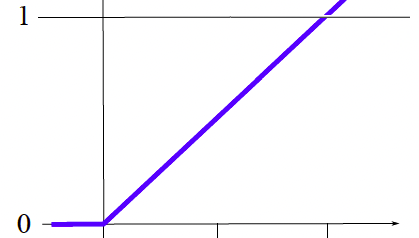
\includegraphics[scale=.4]{./images/relu.png}
\caption[Scott Hotton.]{Graph for the rectified linear or ``ReLU'' activation function.}
\label{relu}
\end{figure}

A special case of a piecewise linear activation function is a \emph{rectified linear unit} or \glossary{ReLU activation function}. The terminology comes from electronics where rectifiers are often used to truncate the negative part of an alternating current to produce a direct current. They cut off all negative values, replacing them with a 0, and leave the weighted input unchanged otherwise (see figure \ref{relu}).\footnote{The rule can be even more concisely stated as the maximum value between 0 and $n_k$, or $\mbox{max}(0,n_k)$.} Thus, they are a piecewise linear function with no upper bound:
\begin{eqnarray*}
a_k = f(n_k) =  
\left\{
      \begin{array}{clc}
                  0      & {\rm if} &   n_k\; \leq \; 0          \\  
              n_k  &  &  \mbox{otherwise}	
      \end{array} 
\right.
\end{eqnarray*}
ReLU has a number of useful properties that have made it extremely popular since the deep learning revolution of the 2010s (section \extref{deep_revolution}). To fully appreciate these advantages it helps to compare it to the piecewise linear activation function, which is in turn similar to the sigmoid activation function, discussed below. Piecewise linear and sigmoid activation functions are only really responsive to inputs between their upper and lower bounds. For large weighted inputs, they just max out at some number, like 1, limiting their expressive power. Whatever large input you throw at them, they always just output $1$. But ReLU can take on \emph{any} positive value, which gives it greater representational power. This in turns makes it more useful in training deep networks.\footnote{The derivative goes to 0 for large values of sigmoids, and that makes the derivative drop to  0, which prevents that node from contributing to learning due to the way errors are ``back-propagated.''  See chapter \extref{ch_lms_backprop} and the discussing of vanishing gradients. Also, the derivative is $0$ for $n_k <= 0$, and $1$ otherwise, except at $0$ (the point of discontinuity), where the derivative is not defined.  A helpful discussion from Leo Dirac that outlines other virtues of ReLU is here: \url{https://youtu.be/S27pHKBEp30?t=1165}. }  On the other hand, the clipping at $0$ is nice, because it maintains a non-linearity (many layers of unclipped linear nodes are mathematically equivalent to one layer of linear nodes, so additional layers don't help). The clipping also removes all negative activations, making overall activation in a large network more sparse, so that different inputs produce nicely distinct activation patterns. In fact, multiple varieties of ReLU function are now available, in particular ``GeLU'', which allows some representation of negative values, is also easy to compute, and has well-defined derivative for every weighted input.  In Simbrain, a ReLU unit can be approximated with a linear activation function whose \emph{lower bound} is 0 and whose \emph{upper bound} is a large number.

\section{Sigmoid Activation Functions}

% Reference to sigmoid's use in Stroop model (see 2009 section on "AttentionStroop")
% Also see "ossification" in Elman ``starting small'' paper

A \glossary{sigmoid activation function} can be thought of as a smoothed version of a piecewise linear activation function. The sigmoid functions get their name from the Greek letter for ``s'', and their graphs are sometimes called ``s-curves'' because they resemble a stretched-out letter ``s''. This is directly visible in figure \ref{activationFunctions}. As weighted inputs increase, the activation approaches the upper value $u$, which is usually $1$. As weighted inputs decrease, the activation approaches the lower value $\ell$, which is usually $0$ or $-1$. When weighted inputs are near the inflection point of the function at 0, activation changes rapidly. Since outputs are always ``squeezed'' between $u$ and $l$, it is sometimes called a ``squashing function.''

  Sigmoid functions can be used to describe natural processes that involve a continuous increase from one value to another. Suppose a bacterium is placed in a Petri dish and we observe how quickly bacteria grow in the dish. At first, the population grows slowly. It then rapidly expands in a neighborhood of the inflection point. As the population begins to fill the dish, the population size levels off, or plateaus. Something similar happens to the firing rate of a neuron as it receives more input currents. The firing rate rises slowly, then rapidly, and then approaches a maximum value.
 % Add more details and references?  Put a bacterium in a petri dish. Close to low value, far from high value. Not much in first hour. Doubling time of 5 minutes. Dividing every 10 minutes. Early stage corresponds to exponential growth. After inflection point exponential decay. // Scott chose  fruit example because the curves are _really_ well modeled by Sigmoid. The bacteria case is more famous but has a bit of noise in there once the dish gets filled up.

Sigmoid activation functions are notable for being differentiable everywhere. If you have not taken calculus, this intuitively means that the function smoothly changes everywhere; there are no discontinuous breaks or hard edges. Notice that the threshold and piecewise linear activation functions in figure \ref{activationFunctions} are not differentiable everywhere. The threshold function has a discontinuity at the threshold value, and the piecewise linear function does not change smoothly at the truncation points $(u,u)$ and $(\ell,\ell)$. The ReLU function is discontinuous at $(0,0)$. The differentiability of the function means that the derivative can be used, which in turn allows certain operations to be performed on sigmoidal nodes that would not otherwise be possible. This led to one of the major innovations in the history of neural networks: the move from linear networks (networks of nodes using linear activation functions) to networks using sigmoidal nodes, which could be trained using backpropagation. This in turn led to an increase in the use of neural networks in the 1980s (see chapter \extref{ch_history}). 

   We will not focus on how to compute a sigmoid function here (the function can be computed in several different ways). We focus on 
the qualitative properties of sigmoid functions. However, to give a flavor of 
the idea, here is one common way by which some sigmoid functions can be 
computed: 
\begin{eqnarray*}
a_k = f(n_k) = \frac{1}{1+e^{-4\, m\, n_k}}
\end{eqnarray*}
(Note that this version of the function incorporates a slope parameter $m$ but not an adjustable upper or lower value. Adding $u$ and $\ell$ parameters would make the function even more complex). This version of the sigmoid function is often called a ``logistic function.''  There are other versions of the sigmoid function, for example, one based on the arctangent function from trigonometry, and another based on the hyperbolic tangent function.\footnote{In Simbrain this function is captured by the ``Sigmoidal (Discrete)'' update rule. Different implementations of the function can be selected within Simbrain.} 
% The 4 is there so that the derivative ends up being m
% logit function.... inverse of logistic?  Shows in logistic regression. All that stuff with link functions and generalized linear model might be worth mentioning here.

In general, we need three values to specify a sigmoid function. We 
need its upper bound, $u$, its lower bound, $\ell$, and a positive slope, $m$. 
For the formula above, $(u,\ell) = (1,0)$ and $m$ can have any positive value.
When the weighted input to a sigmoidal function equals $0$, the resulting activation will be exactly half way 
between the upper and lower bounds, \ie $(u + \ell)/2$, or in this case $(1+0)/2 = .5$. 
The point $(0,  (u + \ell)/2)$ on the graph of the sigmoid function is called the {\em 
inflection point} of the function. Each sigmoid function is symmetrical about
its inflection point. The value of $m$ is the slope of the tangent line to the 
graph of the sigmoid function at the inflection point. In other words, $m$ 
tells us how steeply the graph of a sigmoid function rises.

   As the weighted input is increased indefinitely above $0$, the value of a 
sigmoid function converges to its upper bound $u$. As the weighted input is 
decreased indefinitely below $0$, its value converges to its lower bound $\ell$.
The larger $m$ is, the more rapidly the sigmoid function converges to its 
bounds. Figure \ref{activationFunctions} shows the graph of a sigmoid function with 
$(u,\ell,m) = (1,0,1)$. 

As the slope parameter is varied, the shape of the sigmoid function changes. When the slope is
large or ``steep'', the sigmoid will begin to look like the threshold function. When the slope is near $0$, it will begin to look more like a linear function.